\documentclass[10pt]{article}
\usepackage{amsmath}
\usepackage{listings}
\usepackage{graphicx}
\usepackage{float}
\usepackage{tabularx}
\graphicspath{ {./images/} }
\begin{document}
{\centering
    CSU44061 Machine Learning - Week 8
    \par
    Samuel Petit - 17333946
    \par
    Code for all questions provided in the appendix.
}
\section*{Question i}
\subsection*{Part a}
In order to do so there are 2 problems to solve:
- knowing how many iterations to apply the kernel within the image (for columns and rows)
- For each iteration, compute the resulting value to place in the output

To do so, I start by computing both:
\begin{equation*}
    rows = \# rows_{image} - \# rows_{kernel} + 1
\end{equation*}
\begin{equation*}
    columns = \# columns_{image} - \# columns_{kernel} + 1
\end{equation*}

Then, given that both $rows$ and $columns$ are positive numbers, we know
the amount of positions to place the kernel within the image on both the x and y axis.

The first step is then to iterate over both ranges, that is:
\begin{lstlisting}
x_positions = len(image) - len(kernel) + 1
y_positions = len(image[0]) - len(kernel[0]) + 1
# Make sure kernel and image sizes are valid
assert x_positions > 0 and y_positions > 0, 
        "image should not be smaller than kernel"
# Iterate over kernel positions within the image
for i in range(x_positions):
    for j in range(y_positions):
        # Compute the output point here
\end{lstlisting}

Let's now look at the second problem to solve, that is, given a certain x and y
iteration (here represented as i and j), compute the resulting value to position
in the output matrix.

To do so, I iterate over the kernel matrix rows and columns such as to compute:

\begin{equation*}
    output_{i,j} = \sum_{k = 0}^{\#kernel_{rows}}\sum_{l = 0}^{\#kernel_{columns}} kernel^{(k,l)} * image^{(i + k, j + l)}
\end{equation*}

That it, for each point in the kernel, we multiply it to its corresponding point (using the offset
of i and j), once we have done so for all kernel points we have the result value for the
point ${i,j}$ of the output matrix.

In code this looks like:
\begin{lstlisting}
sum = 0
for k in range(len(kernel)):
    for l in range(len(kernel[0])):
        sum = sum + (kernel[k][l] * image[i + k][j + l])
\end{lstlisting}

Finally, all we need to do now is use this sum to form the current output row and
finally use the row to build the output matrix. All together:

\begin{lstlisting}
def convolutional_layer(image, kernel):
    x_positions = len(image) - len(kernel) + 1
    y_positions = len(image[0]) - len(kernel[0]) + 1
    assert x_positions > 0 and y_positions > 0, 
            "image should not be smaller than kernel"
    result = []
    for i in range(x_positions):
        row = []
        for j in range(y_positions):
            sum = 0
            for k in range(len(kernel)):
                for l in range(len(kernel[0])):
                    sum = sum + (kernel[k][l] * 
                                image[i + k][j + l])
            row.append(sum)
        result.append(row)
    return result
\end{lstlisting}

\subsection*{Part b}
I chose the picture of a triangle found online:

\begin{center}
    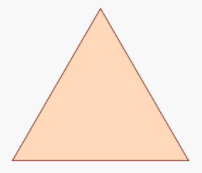
\includegraphics[scale=0.3]{triangle.PNG}
\end{center}

Using the code provided in the assignment and the above picture as an input.
I can apply the 2 provided kernels to my image, we obtain the following
outputs:
\vspace{5mm} %5mm vertical space
Kernel 1:
\begin{center}
    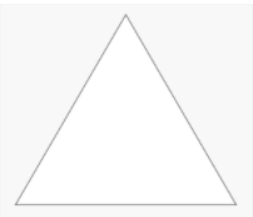
\includegraphics[scale=0.3]{ml_triangle_1.PNG}
\end{center}

\vspace{5mm} %5mm vertical space
Kernel 2:
\begin{center}
    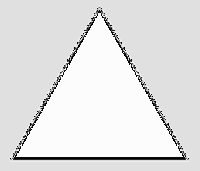
\includegraphics[scale=0.3]{ml_triangle_2.PNG}
\end{center}

\section{Question ii}
\subsection*{Part a}
The downloaded code uses the following ConvNet code:
\begin{lstlisting}
model.add(Conv2D(16, (3,3), padding='same',
        input_shape=x_train.shape[1:],activation='relu'))
model.add(Conv2D(16, (3,3), strides=(2,2), 
                    padding='same', activation='relu'))
model.add(Conv2D(32, (3,3), padding='same', 
                                    activation='relu'))
model.add(Conv2D(32, (3,3), strides=(2,2),
                    padding='same', activation='relu'))
model.add(Dropout(0.5))
model.add(Flatten())
model.add(Dense(num_classes, activation='softmax',
            kernel_regularizer=regularizers.l1(0.0001)))
\end{lstlisting}

We notice a list of sequential steps are added, in order we find:

\begin{itemize}
    \item A 2D Convolution Layer which use 16 filters to learn from. a kernel size of 3x3,
    it also uses padding such as to make outputs the same dimensions as the input, finally
    it also uses 'relu' validation (or rectified linear activation function 
    ) is a method which will map the output to 0 if it is negative.
    \item We then find another 2D Convolution Layer with 16 filters,
    3x3 size, uses padding to keep the same output size and 'relu' activation. The
    difference being that it uses a Stride of size 2x2 such as to downsample
    (it determines how much the window moves by - the default being 1x1)
    \item We then find the exact same 2 steps as we've seen above, in the
    same order with the difference that the filter size is set to 32 instead of 16.
    \item We then find a Droupout step, which sets randomly input values to 0
    with a rate of 0.5 here. This helps to prevent overfitting. It will also
    update non-0 values such as to keep the sum of values consistent.
    \item We then have a Flatten step which simply maps the data to be flat
    \item The final step is a Dense step which is a step for densely connected neural network layers,
    it uses the activation function provided such as to form its output. It uses 10 units (or classes) as specified
    in the downloaded code, L1 regularisation and the activation function is set to
    'softmax' which outputs the values of a probability density function.
\end{itemize}

\subsection*{Part b}
\subsubsection*{Section i}
By simply running the program and reading the output from the
console we find the metrics required by the question:

\begin{itemize}
    \item This model has a total of: 37,146 parameters
    \item The layer with the most parameters is the Dense layer,
    which has 20,490 parameters.
    \item When I ran the code I found that the accuracy on the
    test data was of 0.5, on the train data I obtain an accuracy
    of 0.62. We find that the accuracy does drop by some considerable
    amount compared with the train data ($0.62 - 0.5 = 0.12$), however that makes sense
    as the test data is data the model hasn't seen before, unlike the train.
\end{itemize}

I trained a DummyRegressor model to use as a baseline model for comparison.
This model predicts the most commonly seen value, it is very
straightforward to train:
\begin{lstlisting}
    dummy_model = DummyRegressor().fit(x_train, y_train)
\end{lstlisting}

I then use the same methods as included in the provided code to
obtain an accuracy metric, we find the that baseline model
has an accuracy of 0.1 for both the test and train data. We can 
clearly confirm that our previous model is doing very well in comparison, with an accuracy increase of
$0.5 - 0.1 = 0.4$ on the test data and $0.62 - 0.1 = 0.52$ on the test data.

\subsubsection*{Section ii}
The graph we obtain the history variable in the provided code is the following:

\begin{center}
    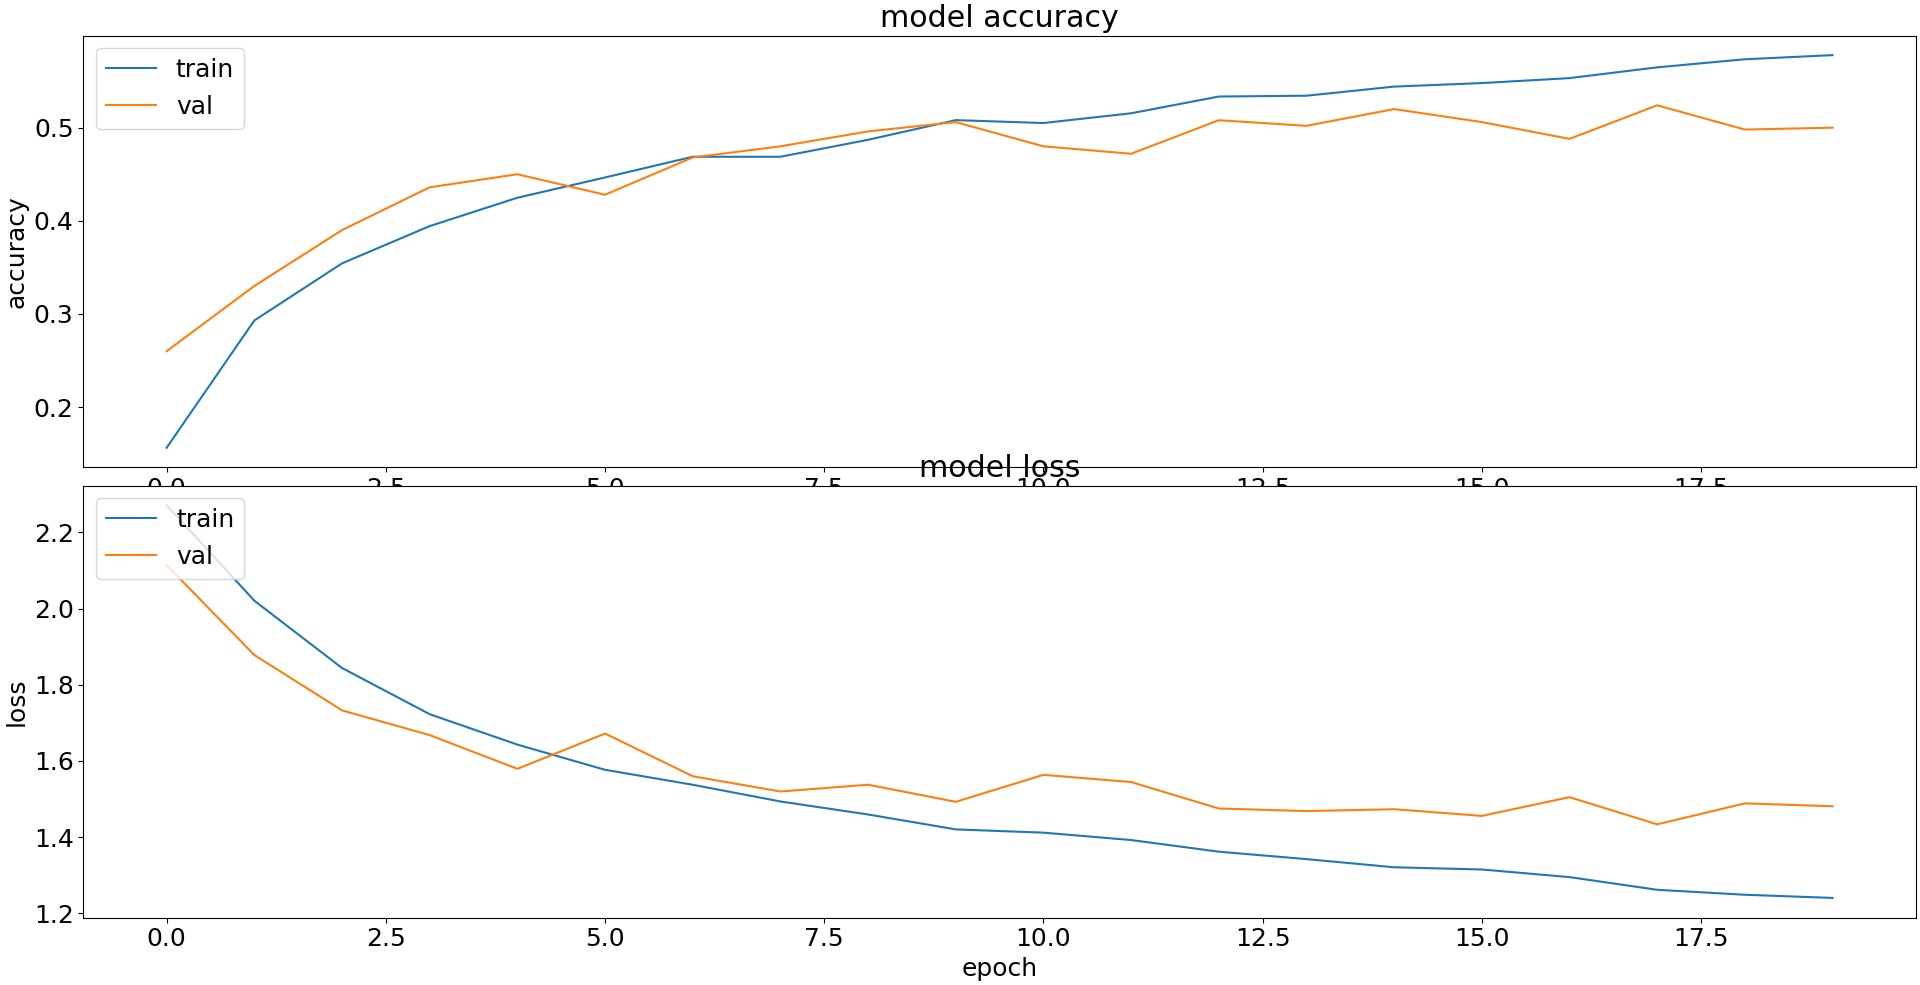
\includegraphics[scale=0.3]{default_5k.png}
\end{center}

Looking at the second part of the graph which plots the loss on the y axis and epoch on the x axis
can be used to make some observations about over and underfitting.
We notice that during the first few epoch (training iterations)
the loss reduces by a noticeable amount quite fast. We could say that
the model was underfitting towards the start and started tuning more
parameters as we increase the epoch number.

However, we get to a point where the loss somewhat stabilises and starts tu fluctuate, becoming
quite unpredictable (it seems to have a high variance). We notice a form of overfitting
where we continue training the model and tuning parameters with no gain in the models performance.

\subsubsection*{Part iii}
Training this same model using bigger amounts of training data
points, I measure the training time and accuracy for each of these
models. We obtain the following metrics:

\vspace{5mm} %5mm vertical space
\begin{center} \begin{tabular}[h]{cccc}
    Train size & Train time & Accuracy train & Accuracy test  \\
    5K         & 41.17s     & 0.63           & 0.49            \\
    10K        & 81.21s     & 0.67           & 0.56            \\
    20K        & 158.01s    & 0.69           & 0.62            \\   
    40K        & 307.86s    & 0.72           & 0.68            \\
\end{tabular} \end{center}

Looking strictly at these metrics we find that doubling the train size
results in roughly double the training time. We notice that both the
accuracy on the train data and the test data increase as the train size increases,
with bigger gaps when increasing from the 5k to 10k than going from 20k to 40k for
example. We notice a pattern here - increasing the train size seems to double the train time,
it will result in greater accuracy values however a decision needs to be made as to
how much training is justified and when to stop training (when the accuracy improvements are
not worth the additional training time). This will heavily depend on the use case, 
perhaps for testing purposes less accuracy is OK, if this were to be used in a business
or important application we likely will want to most accurate model possible.

We obtain the following plots of the "history" variable: 

\begin{figure}[H]    
    \fbox{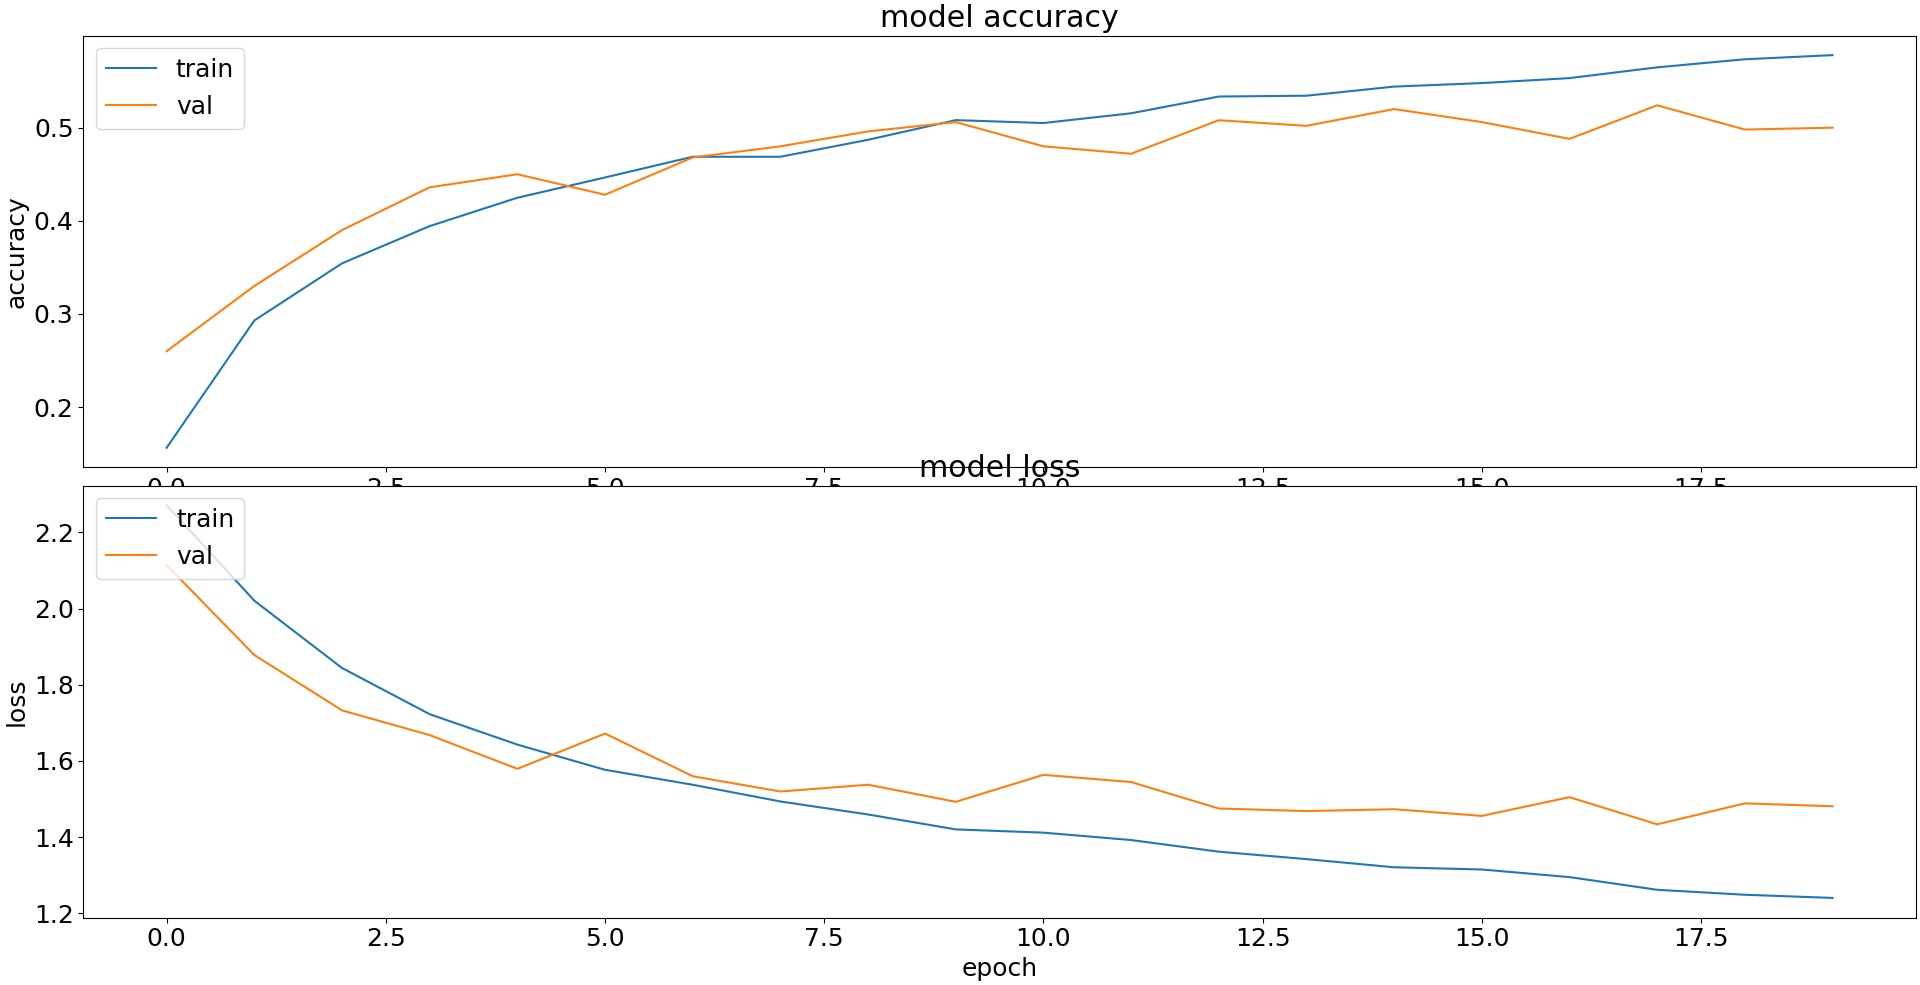
\includegraphics[scale=0.117]{default_5k.png}}   
    \fbox{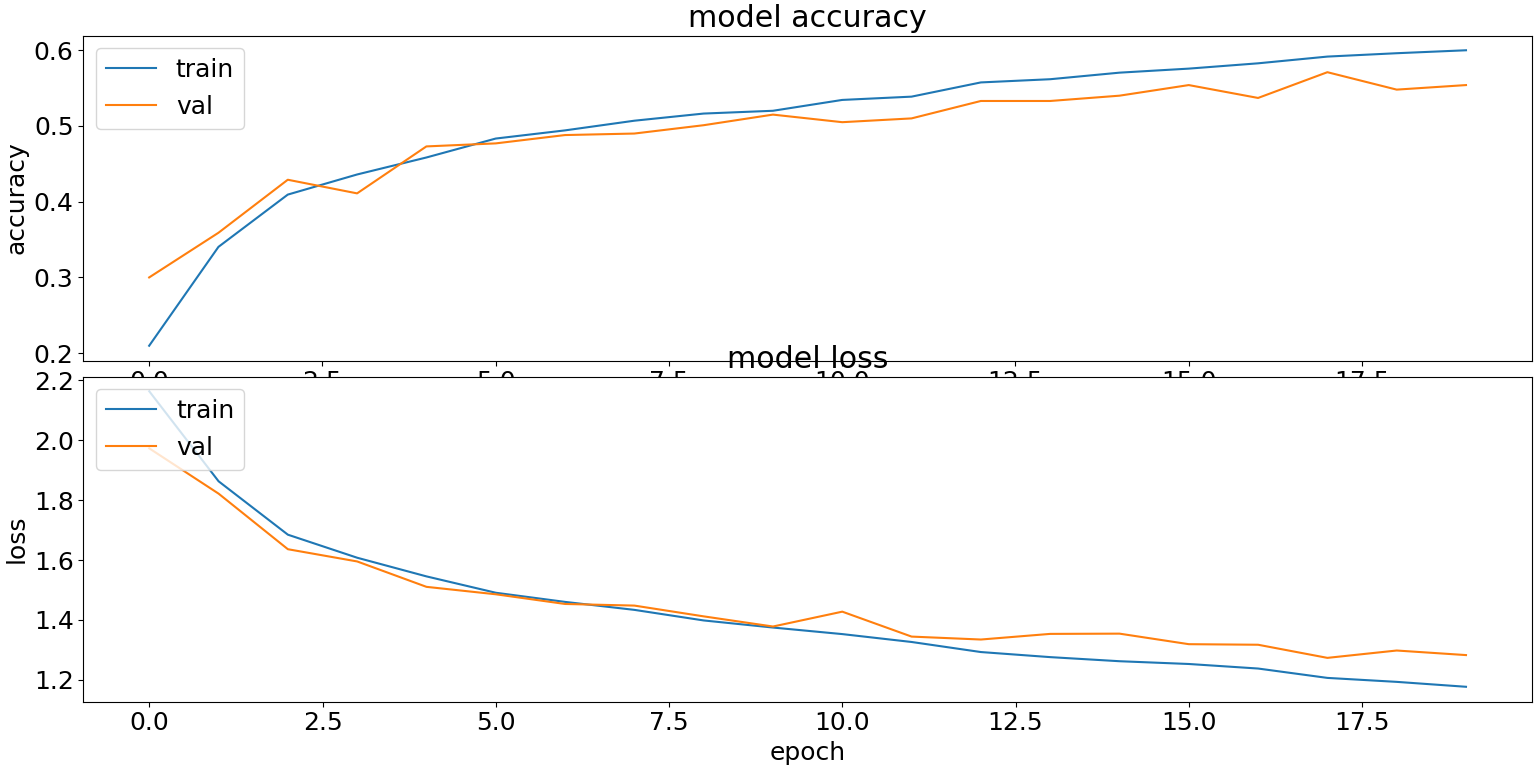
\includegraphics[scale=0.15]{default_10K.png}}   
    \fbox{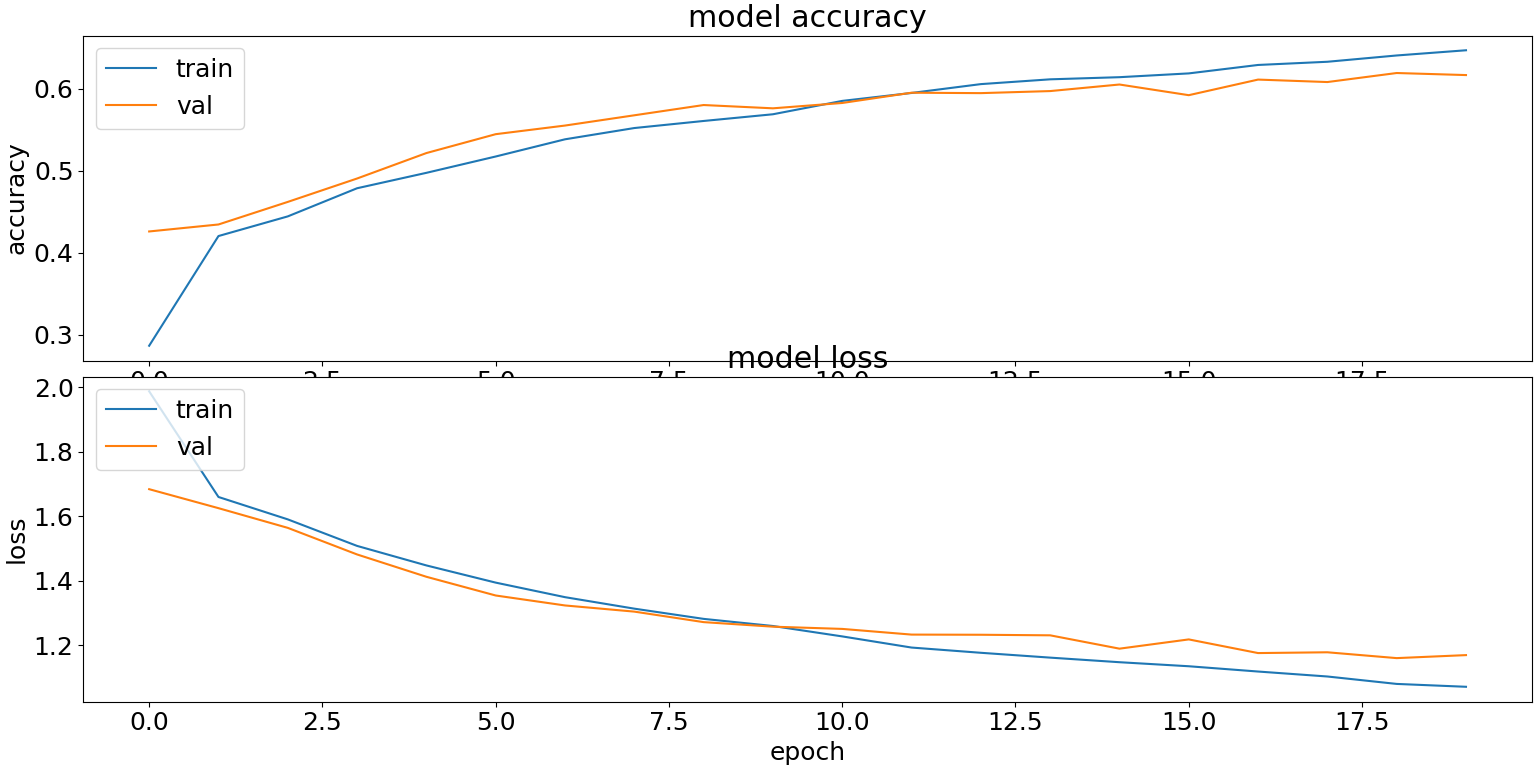
\includegraphics[scale=0.15]{default_20K.png}}
    \fbox{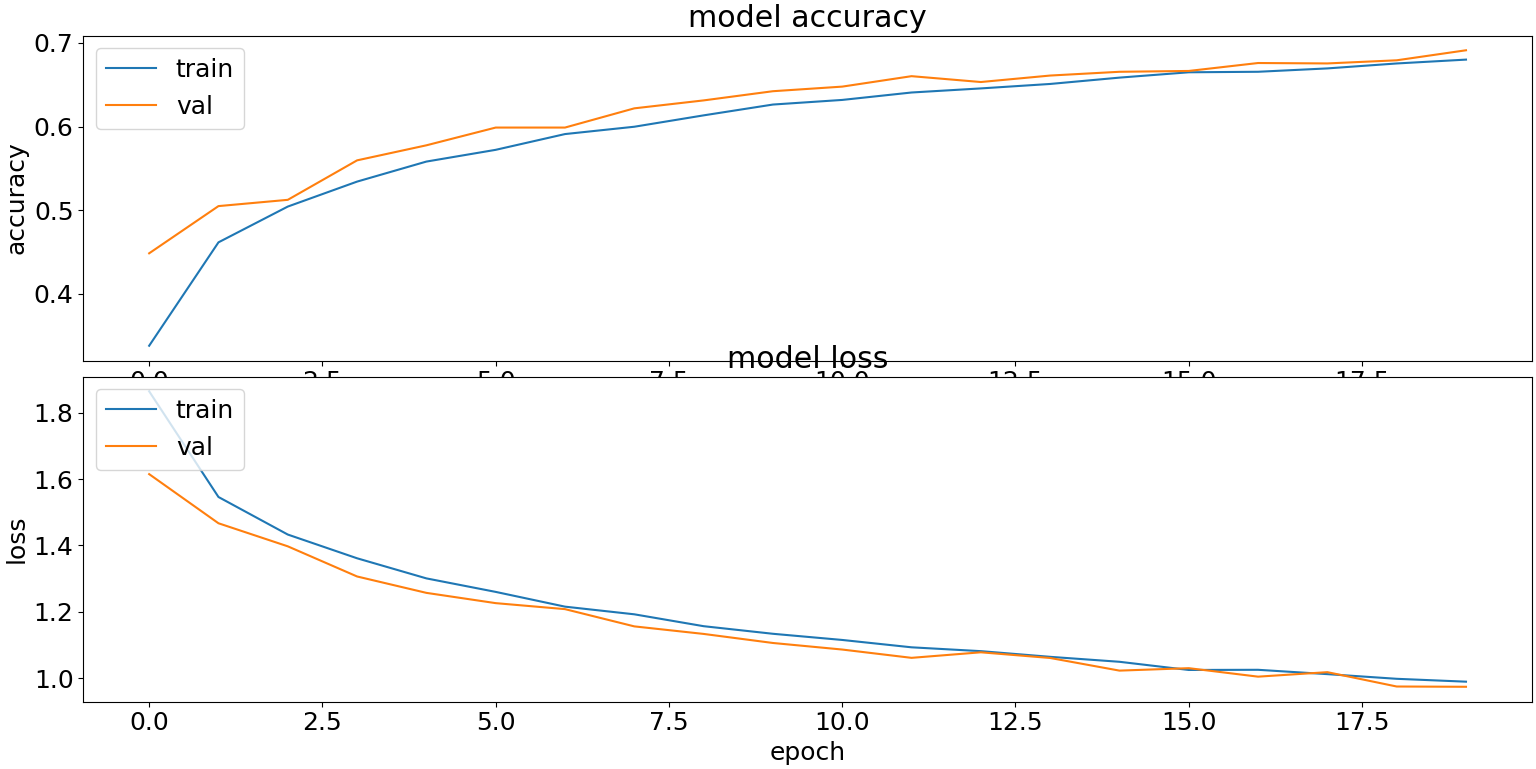
\includegraphics[scale=0.15]{default_40K.png}}
\end{figure}

These plots are in order, going from the top left to the right, then down left to the right.
They represent the history plots for the above sizes, 5K, 10K, 20K and 40K respectively.

The main thing we notice from these plots is that jumps in accuracy based on the loss
or loss against the epoch iteration are much smoother with higher training sizes, we notice
that using a train size of 5K will result in quite big spikes while the size of 40K
is a much smoother with barely any spikes. This is explained by the bigger
training size which makes the accuracy computation much more predictable as there are many more data points used. 

\subsubsection*{Part iv}
Using a variety of weight parameters for the L1 regularisation of this model, I train a model using a 5K train size, every time
recording the accuracy on the training and test data, we obtain the following metrics:

\vspace{5mm} %5mm vertical space
\begin{center} \begin{tabular}[h]{ccc}
    Loss parameter & Accuracy train & Accuracy test  \\
    0.0001 & 0.49           & 0.62            \\
    0.01   & 0.44           & 0.48            \\
    0.1    & 0.37           & 0.38            \\   
    0.5    & 0.29           & 0.30            \\
    0      & 0.50           & 0.65            \\
    2      & 0.1            & 0.1             \\
    10     & 0.1            & 0.1             \\
    100    & 0.1            & 0.1             \\
\end{tabular} \end{center}

We notice interesting behaviors in accuracy in both test and train predictions
as the loss parameter is varied.
To start, we notice that as the loss parameterbecomes 2 or more there is a constant
accuracy in both the train and test data to be 0.1 - this is the same value we found in our
dummy model which predicted the most frequent value earlier ! We can conclude a loss term over
2 will make the weighting too big and cause this model to predict the most frequent value always.

Then, looking at the range of loss between 0.0001 - 0, we notice that the accuracy on the train predictions
fall down from 0.49 to 0.29 and spikes back up to 0.5 when the loss is 0. A loss value of 0
will make the regularisation to be ignored, we find very similar results using no regularisation and using a value of
0.0001.

We notice the exact same trend on the accuracy for the test data - however numbers are higher for the train accuracy
as the test accuracy - this makes sense as the test dataset is data that wasn't used to train the model
thus we can expect lower accuracy values.

\subsection*{Part c}
\subsubsection*{Part i}
As I understood the question, I modified the ConvNet to use 2 convolutional layers
using the "same" parameter of sizes 16 and 32, followed by a "max-pooling" layer,
thus removing the layers which used strides. The following layers (such as 
density layer, the dropout or the flatten layer) are left untouched.
We are left with the following layers:

\begin{lstlisting}
model.add(Conv2D(16, (3,3), padding='same', 
        input_shape=x_train.shape[1:],activation='relu'))
model.add(Conv2D(32, (3,3), padding='same', 
                                    activation='relu'))
# New layer
model.add(MaxPooling2D((2,2)))
# Following lines remain the same
model.add(Dropout(0.5))
model.add(Flatten())
model.add(Dense(num_classes, activation='softmax',
kernel_regularizer=regularizers.l1(0.0001)))
model.compile(loss="categorical_crossentropy",
                optimizer='adam', metrics=["accuracy"])
\end{lstlisting}

We will examine outputs of this new architecture of layers in the following question.

\subsubsection*{Part ii}
Using the model from the previous section, a training size of 5K and the original loss
parameter of 0.0001, we can train a new model. Reading the output from the console
we obtain the following values:

\begin{itemize}
    \item Train time: 65.16s
    \item Total parameters: 87,018
    \item Accuracy test: 0.53
    \item Accuracy train: 0.75
\end{itemize}

Remeber that the original network using the same 5K training size and 0.0001
loss parameter had the following:

\begin{itemize}
    \item Train time: 41.17s
    \item Total parameters: 37,146
    \item Accuracy test: 0.50
    \item Accuracy train: 0.63
\end{itemize}

First of all, we notice a difference in training times, the original model
taking 41s while the new took 65s. I believe that is due to the removal of the two
layers which used strides to downsample the data. Thus we are no longer downsampling
which explains the longer run time.

As of metrics, we find many more parameters (87,018) on the new model, that is
$87018 - 37146 = 49872$ more parameters than our original model! This is quite significant.

Let's see how the added parameters do in terms of accuracy, we notice a small
improvement in test accuracy (improvement of $0.53 - 0.5 = 0.03$) - it isn't a big improvement
but still worth noting.
In terms of the training data though the improvement is slightly more considerable: $0.75 - 0.63 = 0.12$.


\section*{Appendix}
Part i:
\begin{lstlisting}
from PIL import Image
import numpy as np


def convolutional_layer(image, kernel):
    x_positions = len(image) - len(kernel) + 1
    y_positions = len(image[0]) - len(kernel[0]) + 1
    assert x_positions > 0 and y_positions > 0,
                "image should not be smaller than kernel"
    result = []
    # Iterate over possible positions
    for i in range(x_positions):
        row = []
        for j in range(y_positions):
            sum = 0
            # Compute sum for current output point i,j
            for k in range(len(kernel)):
                for l in range(len(kernel[0])):
                    sum = sum + (kernel[k][l] *
                                    image[i + k][j + l])
            row.append(sum)
        result.append(row)
    return result


im = Image.open('triangle.PNG')
rgb = np.array(im.convert('RGB'))
r = rgb[:, :, 0]

kernel1 = np.array([[-1, -1, -1], [-1, 8, -1],
                                        [-1, -1, -1]])
kernel2 = np.array([[0, -1, 0], [-1, 8, -1], 
                                        [0, -1, 0]])

im_k1 = convolutional_layer(r, kernel1)
im_k2 = convolutional_layer(r, kernel2)

Image.fromarray(np.uint8(im_k1)).show()
Image.fromarray(np.uint8(im_k2)).show()
\end{lstlisting}

Part ii:
\begin{lstlisting}
import sys
import time
from sklearn.dummy import DummyRegressor
import numpy as np
import tensorflow as tf
from tensorflow import keras
from tensorflow.keras import layers, regularizers
from keras.layers import Dense, Dropout, Activation,
                            Flatten, BatchNormalization
from keras.layers import Conv2D, MaxPooling2D,
                                LeakyReLU
from sklearn.metrics import confusion_matrix,
                                classification_report
from sklearn.utils import shuffle
import matplotlib.pyplot as plt
plt.rc('font', size=18)
plt.rcParams['figure.constrained_layout.use'] = True

# Model / data parameters
num_classes = 10
input_shape = (32, 32, 3)

# the data, split between train and test sets
(x_train, y_train), (x_test, y_test) =
                    keras.datasets.cifar10.load_data()
# Update this line to change train size (5k,10k,20k,40k)
n = 5000
x_train = x_train[1:n]
y_train = y_train[1:n]
#x_test=x_test[1:500]; y_test=y_test[1:500]

# Scale images to the [0, 1] range
x_train = x_train.astype("float32") / 255
x_test = x_test.astype("float32") / 255
print("orig x_train shape:", x_train.shape)

# convert class vectors to binary class matrices
y_train = keras.utils.to_categorical(y_train,
                                    num_classes)
y_test = keras.utils.to_categorical(y_test, num_classes)

use_saved_model = False
if use_saved_model:
    model = keras.models.load_model("cifar.model")
else:
    model = keras.Sequential()
    model.add(Conv2D(16, (3, 3), padding='same',
        input_shape=x_train.shape[1:], activation='relu'))
    model.add(Conv2D(16, (3, 3), strides=(2, 2), padding='same',
        activation='relu'))  # comment line for part ii c
    model.add(Conv2D(32, (3, 3), padding='same', activation='relu'))
    model.add(Conv2D(32, (3, 3), strides=(2, 2), padding='same',
        activation='relu'))  # comment line for part ii c
    # Uncomment for part ii c
    # model.add(MaxPooling2D((2,2)))
    model.add(Dropout(0.5))
    model.add(Flatten())
    # Change l1 parameter for part b iv
    model.add(Dense(num_classes, activation='softmax',
            kernel_regularizer=regularizers.l1(0.0001)))
    model.compile(loss="categorical_crossentropy",
                  optimizer='adam', metrics=["accuracy"])
    model.summary()

    batch_size = 128
    epochs = 20
    start = time.time()
    history = model.fit(x_train, y_train, batch_size=batch_size,
                        epochs=epochs, validation_split=0.1)
    end = time.time()
    print("time spent training: ", end - start)
    model.save("cifar.model")
    plt.subplot(211)
    plt.plot(history.history['accuracy'])
    plt.plot(history.history['val_accuracy'])
    plt.title('model accuracy')
    plt.ylabel('accuracy')
    plt.xlabel('epoch')
    plt.legend(['train', 'val'], loc='upper left')
    plt.subplot(212)
    plt.plot(history.history['loss'])
    plt.plot(history.history['val_loss'])
    plt.title('model loss')
    plt.ylabel('loss')
    plt.xlabel('epoch')
    plt.legend(['train', 'val'], loc='upper left')
    plt.show()

print("Trained model: train data perf")
preds = model.predict(x_train)
y_pred = np.argmax(preds, axis=1)
y_train1 = np.argmax(y_train, axis=1)
print(classification_report(y_train1, y_pred))
print(confusion_matrix(y_train1, y_pred))

print("Trained model: test data perf")
preds = model.predict(x_test)
y_pred = np.argmax(preds, axis=1)
y_test1 = np.argmax(y_test, axis=1)
print(classification_report(y_test1, y_pred))
print(confusion_matrix(y_test1, y_pred))

# Dummy model
dummy_model = DummyRegressor().fit(x_train, y_train)

print("Dummy model: train data perf")
# Display train prediction performance
preds_dummy = dummy_model.predict(x_train)
y_pred_dummy = np.argmax(preds_dummy, axis=1)
y_pred_dummy1 = np.argmax(y_train, axis=1)
print(classification_report(y_pred_dummy1, y_pred_dummy))
print(confusion_matrix(y_pred_dummy1, y_pred_dummy))

print("Dummy model: test data perf")
# Display test prediction performance
preds_dummy = dummy_model.predict(x_test)
y_pred_dummy = np.argmax(preds_dummy, axis=1)
y_pred_dummy1 = np.argmax(y_test, axis=1)
print(classification_report(y_pred_dummy1, y_pred_dummy))
print(confusion_matrix(y_pred_dummy1, y_pred_dummy))
\end{lstlisting}
\end{document}
